\documentclass{article}

% Language setting
% Replace `english' with e.g. `spanish' to change the document language
\usepackage[english]{babel}
\usepackage{geometry}
\usepackage{algorithm}
\usepackage[noend]{algpseudocode}

% Set page size and margins
% Replace `letterpaper' with `a4paper' for UK/EU standard size
 \geometry{
 a4paper,
 total={170mm,257mm},
 left=20mm,
 top=20mm,
 }
% Useful packages
\usepackage{amsmath}
\usepackage{graphicx}
\usepackage[colorlinks=true, allcolors=blue]{hyperref}

\title{Reasoning and Agents - Coursework 1}
\author{Finlay Ross-Davie}

\begin{document}
\maketitle

\section{Part A}

\subsection{A}

Constraints:

$D = {1,2,3,4,5,6,7,8}$

\begin{equation}
GreaterThan(x,y)
    \begin{cases}
        if \: x > y \: then \: True \\
        otherwise \: False
    \end{cases}
\end{equation}

\begin{equation}
NotEqual(x,y)
    \begin{cases}
        if \: x \neq y \: then \: True \\
        otherwise \: False
    \end{cases}
\end{equation}

\begin{equation}
LessThanEqual(x,y)
    \begin{cases}
        if \: x \leq y \: then \: True \\
        otherwise \: False
    \end{cases}
\end{equation}


C = \{\

$NotEqual(a,b), \forall a, b \in destinations$ \newline
$GreaterThan(h_2,r_1)$ \newline
$GreaterThan(h_3, r_2)$ \newline
$GreaterThan(h_4, r_2)$ \newline
$GreaterThan(h_5, r_3)$ \newline
$GreaterThan(h_3,h_i), \forall i \in \{1,2,4,5\}$ \newline
$LessThanEqual(r_i,5), \forall i \in \{1,2,3\}$ \newline 

\}\

\subsection{B}
Order 1 features a ternary constraint 

$(h_1, r_1, r_2) = (h_1 = max\{r_1, r_2\} + 1)$ \newline

$c = $\{\
$(R, r_1) = (R = r_1)$ \newline
$(R, r_2) = (R = max\{R, r_2\})$ \newline
$(h_1, R) = (h_1 = R+1)$ \newline
\}\

\subsection{C}

\begin{figure}[ht]
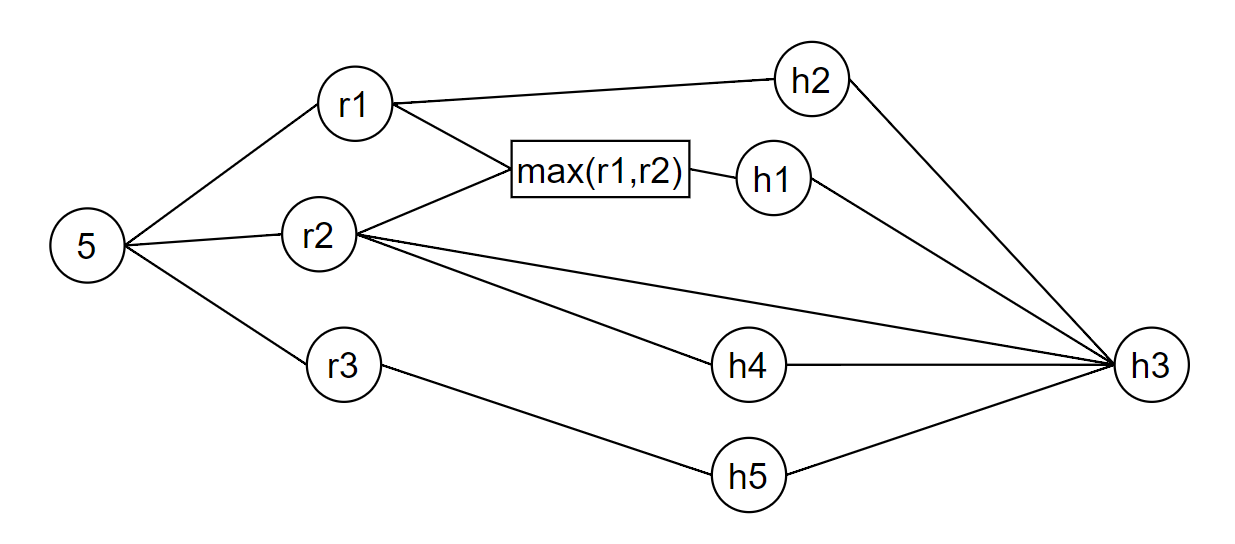
\includegraphics[width=8cm]{ConstraintGraph.png}
\centering
\end{figure}




\end{document}